\documentclass{beamer}
%
% Choose how your presentation looks.
%
% For more themes, color themes and font themes, see:
% http://deic.uab.es/~iblanes/beamer_gallery/index_by_theme.html
%
\mode<presentation>
{
  \usetheme{Warsaw}      % or try Darmstadt, Madrid, Warsaw, ...
  \usecolortheme{crane} % or try albatross, beaver, crane, ...
  \usefonttheme{default}  % or try serif, structurebold, ...
  \setbeamertemplate{navigation symbols}{}
  \setbeamertemplate{caption}[numbered]
} 

\usepackage[english,serbian]{babel}
\usepackage[utf8]{inputenc}
\usepackage[T2A]{fontenc} % enable Cyrillic fonts
\usepackage{currvita}
\usepackage{listings}
\usepackage{lipsum}

\title[PHP]{Programski jezik PHP}%short, full
\author[Vučković, Ivanović, Simić, Stevović]{Đorđe Vučković, Tamara Ivanović,\\ Petar Simić, Stefan Stevović}
\institute{\small{Seminarski rad u okviru kursa\\Metodologija stručnog i naučnog rada\\ Matematički fakultet}}
\date{Maj, 2019.}

\begin{document}

\begin{frame}
  \titlepage
\end{frame}

% Uncomment these lines for an automatically generated outline.
%\begin{frame}{Outline}
%  \tableofcontents
%\end{frame}

%%%%%%%%%%%%%%%%%%%%%%%%%%%%%%%%%%
\section{Uvod}

\begin{frame}{Uvod}

\begin{itemize}
  \item Hypertext preprocessor
  \item Skriptni jezik opšte namene
  \item Nestriktna semantika
  \item U prvih 6 jezika na GitHub-u
  \item Veliki broj radnih okuženja
  \item ,,Learning PHP", ,,PHP Cookbook", ,,Programming PHP"
  
\end{itemize}

\end{frame}

%%%%%%%%%%%%%%%%%%%%%%%%%%%%%%%%%%
\section{Programski jezik PHP}
\subsection{Istorijski razvoj}
\begin{frame}{Istorijski razvoj}
	\begin{itemize}
		\item Rasmus Lerdorf, 1994. godina
		\item Niz C skriptova - PHP Tools
		\item FI (eng. Forms Interpreter)
		\item 1996. - Alat FI evoluirao u programski jezik PHP/FI
		\item Zeev Suraski i Andi Gutmans - redizajnirano PHP/FI jezgro, novi programski jezik Hypertext Preprocessor
		\item Zend Engine - modularnost, leksička analiza, upravljanje memorijom...
		\item PHP 4.0 - poboljšane performanse, podrška HTTP sesijama, novi jezički konstrukti
	
	
	\end{itemize}
    
\end{frame}

%%%%%%%%%%%%%%%%%%%%%%%%%%%%%%%%%%
\subsection{Mogućnosti PHP-a}
\begin{frame}{Mogućnosti PHP-a}
    	\begin{itemize}
		\item Posebno pogodan za veb razvoj na strani servera
		\item Koristiti se na mnogim operativnim sistemima kao i na sistemima za upravljanje relacionim bazama podatataka		
		\item Pisanje skriptova komandne linije
		\item Aplikacije grafičkog korisničkog interfejsa na strani klijenta
		
		% slika za skriptovanje
		\begin{figure}[h!]
                \begin{center}
                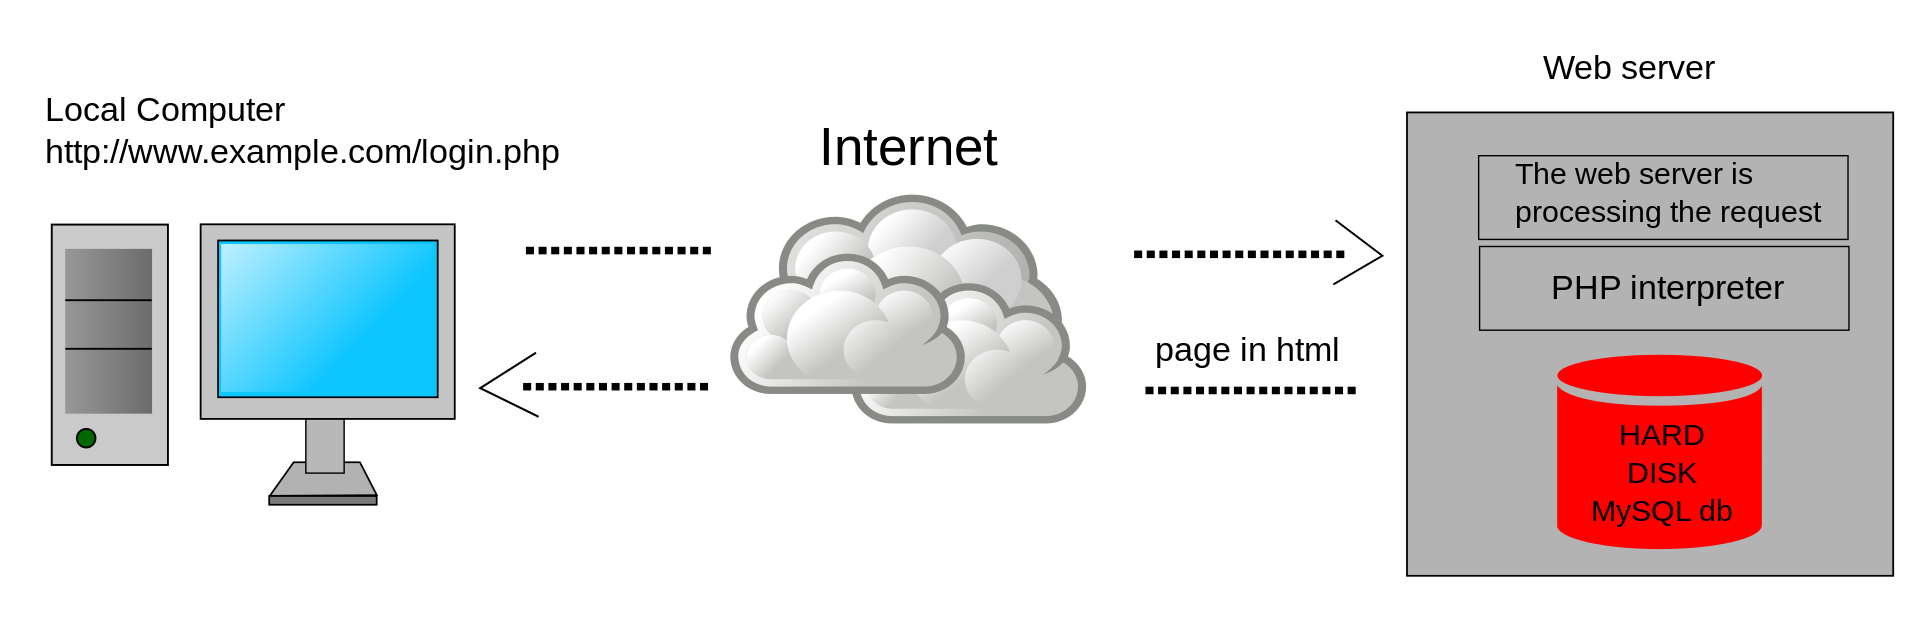
\includegraphics[scale=0.10]{primer_serverskog_skriptiranja.png}
                \end{center}
                \caption{Primer serverskog skriptiranja}
                \label{fig:primer_serverskog_skriptiranja}
                \end{figure}
		
		\item Za naprednije korišsćenje nudi dobro defnisan i dokumentovan način za pisanje ekstenzija u C ili C++
	\end{itemize}	
\end{frame}

%%%%%%%%%%%%%%%%%%%%%%%%%%%%%%%%%%%%
\subsection{Implementacije PHP-a}
\begin{frame}{Implementacije PHP-a}
    	\begin{itemize}
		\item Zend Engine pozananta kao PHP, originalna i najraširenija implementacija   
		\item HHVM(HipHop Virtual Machine) 
		\item Parrot
		\item Phalanger	
		\item Kuercus
	\end{itemize}				
\end{frame}

\subsection{Podržane paradigme}
\begin{frame}{Podržane paradigme}
     	\begin{itemize}
		\item Od vezije 5.0 ima podršku za objektno-orijentisano programiranje  
		\item Podržava funkcije prve klase
		\item Od verzije 5.3 uvedena je i podrška za anonimne funkcije	
		\item Od verzije 5.4 je dodata mogućnost povezivanja zatvaranja sa opsegom objekta
		\item Zbog gore navedenih osobina opravdava pripadanje funkcionalnoj paradigmi
	\end{itemize}
\end{frame}


%%%%%%%%%%%%%%%%%%%%%%%%%%%%%%%%%%%%%%
\subsection{Najpoznatija okruženja}
\begin{frame}{Najpoznatija okruženja}
    	\begin{itemize}
		\item Laravel
			\begin{itemize}
				\item Brzina
				\item MVC
			\end{itemize}
		\item CodeIgniter
			\begin{itemize}
				\item Bezbednost
				\item Sveobuhvatna dokumentacija
			\end{itemize}
		\item Symfony
			\begin{itemize}
				\item Podrška
				\item Fleksibilnost
			\end{itemize}
	\end{itemize}
\end{frame}

%%%%%%%%%%%%%%%%%%%%%%%%%%%%%%%%%%%%%%%
\subsection{Instalacija na Windows OS}

\begin{frame}{Instalacija na Windows OS}
	\begin{itemize}
		\item WAMP server
		\item http://www.wampserver.com/en/
	\end{itemize}


% Commands to include a figure:
%\begin{figure}
%\includegraphics[width=\textwidth]{your-figure's-file-name}
%\caption{\label{fig:your-figure}Caption goes here.}
%\end{figure}

\end{frame}

\subsection{Instalacija na Linux OS}

\begin{frame}{Instalacija na Linux OS}
	\begin{figure}
	\includegraphics[width=\textwidth]{linux_instalacija.png}
	\caption{\label{fig:your-figure}Instalacija na linux-u}
	\end{figure}
\end{frame}

%%%%%%%%%%%%%%%%%%%%%%%%%%%%%%%%%%%%%%%%


%%%%%%%%%%%%%%%%%%%%%%%%%%%%%%%%%%%%%%%
\subsection{Specifičnosti jezika}
\begin{frame}{Specifičnosti jezika}
    \begin{itemize}
		\item Sintaksa jezika nije strogo definisana
		
		% slika za kod
		\begin{figure}[h!]
                \begin{center}
                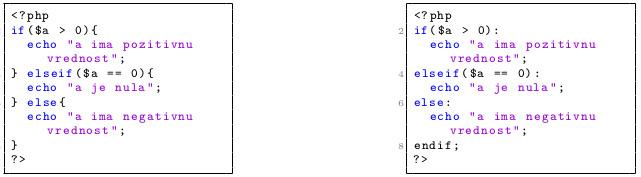
\includegraphics[scale=0.40]{kod.png}
                \end{center}
                \caption{Standardni pristup (levo) i alternativni pristup (desno)}
                \label{fig:kod}
                \end{figure}
                
		\item Upotreba formi
	\end{itemize}
\end{frame}

\begin{frame}{Specifičnosti jezika}
    \begin{itemize}
        \item Klase PDO (PHP Data Object) i DateTime
        
        % slika za datetime
        \begin{figure}[h!]
        \begin{center}
        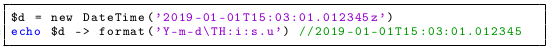
\includegraphics[scale=0.45]{datetime.png}
        \end{center}
        \caption{Primer DateTime biblioteke}
        \label{fig:datetime}
        \end{figure}
        
        \item Upotreba kolačića (eng. cookies)
        \item Sistem za memorisanje objekata distribuirane memorije \\ (eng. Memcached)
    \end{itemize}
\end{frame}


%%%%%%%%%%%%%%%%%%%%%%%%%%%%%%%%%%%%%%%%%
\section{Zaključak}
\begin{frame}{Zaključak}
    \begin{itemize}
    \item Popularan jezik
    \item Velike mogućnosti 
    \item Predstavljene prednosti u odnosu na druge jezike
    \item Trudili smo se da zainteresujemo programere da počnu da se bave PHP-om
    \end{itemize}
\end{frame}


%%%%%%%%%%%%%%%%%%%%%%%%%%%%%%%%%%%%%%%%%
\section{Literatura}
\begin{frame}{Literatura}
    \begin{itemize}
        \item L. Atkinson. Core PHP Programming. Prentice Hall, 2003.
        \item https://www.php.net/manual/
        \item R. Lerdorf and K. Tatroe. Programming PHP. O'Reilly Media, 2002
        \item A. Trachtenberg and D. Sklar. PHP Cookbook, 3rd Edition,  O'Reilly Media, 2014
    \end{itemize}
\end{frame}

\end{document}






